\documentclass[a4paper, 12pt]{article}
\usepackage[utf8]{inputenc}%%seul package à charger~: pour éviter les problèmes sordides d'encodage
\usepackage[rapport, psc]{andre}%%bon eh bien sûr...

\usepackage{makeidx}              %% permet de générer un index automatiquement
\usepackage[style=numeric, backend=bibtex]{biblatex}				%% Utilisé pour la biblio
\usepackage[hidelinks]{hyperref}



\title{Projet Scientifique Collectif X2013 \\INF02~: Synthétiseur automatique de documents \\Rapport final}
\renewcommand{\petittitre}{Projet INF02}
\newcommand{\pyt}[1]{\texttt{#1}}%noms python
\newcommand{\ang}[1]{\textit{#1}}%noms anglais
\author{\membres} %%\membres uniquement avec l'option psc
\date{20 avril 2015}


\index{Réseau sémantique}
\index{Analyse symbolique}
\index{Analyse sémantique}
\index{Réseau de Concepts}

\makeindex
\addbibresource{biblio.bib}
\begin{document}

\titrelong{}


\tableofcontents
\newpage

\section{Rappel du projet}

\subsection{Notre groupe}
\begin{itemize}
 \item Fernandes-Pinto-Fachada Sarah, \textbf{8\textsuperscript{e}} compagnie, section \textbf{équitation};
 \item Schrottenloher André, \textbf{8\textsuperscript{e}} compagnie, section \textbf{escrime};
 \item Angibault Antonin, \textbf{8\textsuperscript{e}} compagnie, section \textbf{escrime};
 \item Hufschmitt Théophane, \textbf{8\textsuperscript{e}} compagnie, section \textbf{escrime};
 \item Cao Zhixing, \textbf{9\textsuperscript{e}} compagnie, section \textbf{escalade};
 \item Boisseau Guillaume, \textbf{6\textsuperscript{e}} compagnie, section \textbf{natation};
\end{itemize}

\subsection{Notre sujet}

\subsubsection{But du projet}
%reprise textuelle

Le but de notre projet était de produire un programme capable d'analyser sémantiquement\index{Analyse sémantique} un texte ayant pour sujet le sport (et plus particulièrement encore le football) de façon à en produire un résumé. Il s'agit là d'une véritable innovation par rapport à l'état actuel du résumé automatique, dans la mesure où les programmes existants se basent prioritairement sur une analyse statistique plus ou moins poussée de fréquence d'apparition des mots pour juger de leur importance~; notre programme s'appuierait plutôt sur le sens pour juger de la pertinence d'un concept et savoir s'il doit le faire figurer ou non dans le résumé final.


\subsubsection{Modules du projet et répartition du travail}
%%reprise textuelle

Pour atteindre cet objectif, plusieurs modules assez indépendants ont pu être identifiés et traités séparément~:

\begin{description}
	\item[Récupération de données] à utiliser pour la création d'un réseau de concepts modélisant la connaissance \textit{a priori} du programme. Responsables~: Théophane Hufschmitt, Guillaume Boisseau.
	\item[Création du réseau de concepts] et remplissage de celui-ci. Il s'agissait ici d'une part de définir sa structure et d'autre part d'y introduire les données nécessaires. Responsables~: André Schrottenloher, Guillaume Boisseau.
	\item[Analyse syntaxique] à l'aide d'outil existants. Il s'agissait de trouver une grammaire capable d'analyser une phrase et d'en faire ressortir les relations de type verbe-objet ou nom-qualificatif. Responsables~: Antonin Angibault, Théophane Hufschmitt, Sarah Fernandes-Pinto-Fachada.
	\item[Réflexion] sur l'utilisation du réseau de concepts et de l'analyse grammaticale pour produire un réseau capable de rendre compte de la compréhension du texte. Responsables~: tous.
	\item[Implémentation] d'un algorithme simple de résumé statistique (basé sur l'algorithme TF-IDF), devant servir de base de comparaison pour tester la qualité des résumés produits par notre algorithme.  Responsable~: Zhixing Cao.
\end{description}

\subsubsection{Outils extérieurs utilisés}

Nous reviendrons sur ces outils et détaillerons au fur et à mesure du rapport.

\begin{itemize}
	\item[WordNet~: ]Dictionnaire permettant d'obtenir la classe grammaticale des mots présents dans le réseau.
	\item[Conceptnet~: ]Grande base de connaissances permettant d'établir la proximité conceptuelle entre différents termes du réseau.
	\item[Freebase~: ]Cette base de connaissances très étendue permet d'identifier les noms propres, par exemple des joueurs de football ou différents stades.
	\item[Natural Language ToolKit (\pyt{nltk})~: ]Divers outils grammaticaux pour l'étude du langage naturel.
	\item Un analyseur syntaxique dont les résultats nous ont été fournis par Systran.
\end{itemize}



\section{Sources de données et traitement de celles-ci}

\subsection{Résumé}

Les données occupent une place essentielle dans notre projet et elles ont revêtu différentes formes.

%%reprise textuelle
Nous utilisons deux sources de données~: des données brutes, sous forme de langage naturel (textes d'articles écrits en anglais), et des données déjà travaillées, le plus souvent mises sous la forme de graphe sémantique.\index{Graphe sémantique}

\begin{definition}[Graphe sémantique]
En première approximation, nous faisons renvoyer la notion de graphe sémantique à un graphe où les nœuds sont étiquetés par des mots et où les arêtes représentent un lien ou expriment une relation entre ces mots.
\end{definition}


\subsection{Données textuelles brutes}

Nous avons récupéré automatiquement des données sur différents sites internet et flux rss, en moyenne 400 articles de sports par jour~; ce qui représentait à la fin du projet plus de 30~000 articles.

%%reprise textuelle
Ces données servent à différents niveaux~:
\begin{itemize}
 \item Dans la création du réseau de concepts (partie suivante)~;
 \item Dans la production de résumés automatiques.
\end{itemize}



\subsection{Traitement de données textuelles}
%%reprise textuelle

Les mots présents dans les articles, pour être reliés à leur signification et décorrélés de leur rôle grammatical, doivent être mis sous forme normale.

\begin{definition}[Forme normale]
La forme normale d'un mot\index{Forme normale} est tout simplement celle qu'il a lorsqu'on le recherche dans le dictionnaire, par exemple~:
\begin{itemize}
 \item Si c'est un verbe, on le met à l'infinitif~;
 \item Au singulier si c'est un nom.
\end{itemize}
Mettre un mot sous forme normale permet de s'intéresser uniquement au sens du mot hors de tout contexte.
\end{definition}


\begin{definition}[Part-of-speech tagger]
Le Part-of-speech tagger\index{Part-of-speech tagger}, abrégé en POS, est un programme, le plus souvent entraîné sur de grandes bases de données, qui permet d'associer à chaque mot dans une phrase une valeur grammaticale.
\end{definition}

\begin{definition}[Concept]
Par le terme de concept\index{Concept}, qui sera constamment réutilisé par la suite, nous entendons~: un mot (adjectif, verbe, nom, nom propre, adverbe) ou un ensemble de mots exprimant une unité sémantique et que l'on peut définir. Par exemple, ``football'' est un concept, tandis que ``if'' pour nous n'en est pas un.
\end{definition}

\`A partir d'articles consacrés au sport (texte brut), les manipulations suivantes permettent de récupérer les noms propres et les concepts sous forme normale\index{forme normale}~:
\begin{itemize}
 \item Découpage du texte en phrases et en mots (\textit{tokens})~;
 \item Utilisation d'un POS, celui de \pyt{nltk}\index{Natural Language ToolKit} par défaut~;
 \item Récupération des noms propres et mise à part de ceux-ci (qui doivent faire plus tard l'objet d'un traitement particulier)~;
 \item Suppression des conjonctions de coordination, pronoms et autres mots qui ne sont pas de véritables concepts~;
 \item Il reste alors des adjectifs, adverbes, noms et verbes. Nous utilisons \pyt{morphy} de WordNet\index{WordNet} à l'intérieur d'un code dédié à la construction de Conceptnet5 (voir partie suivante), pour transformer chaque terme en sa forme normale~;
 \item Les termes restants sont alors tous les concepts auxquels le texte fait appel~;
 \item Nous ne sommes pas à l'abri d'erreurs liées à l'une des étapes. De manière générale, un concept qui apparaît au moins deux fois dans l'ensemble du corpus considéré peut être considéré comme valide.
\end{itemize}

Les noms propres mis à part, nous parvenons à en extraire les noms complets. Dans un texte comme ceux que nous étudions, le nom complet (nom et prénom) n'est souvent mentionné qu'une seule fois, et il faut repérer sans faire d'erreur que le nom propre utilisé seul par la suite renvoie à la même personne.

La récupération des noms propres et concepts sous forme normale permet de nous constituer des listes de termes relatifs au sport. La figure~\ref{fig:conceptsnoms} donne une idée de l'évolution de la taille de ces données. Nous n'avons jamais espéré une exhaustivité, mais il est clair que la croissance observée vers la fin peut être imputée en majeure partie aux données parasites (mots mal orthographiés, erreurs de lecture) et que nous avons, pour ainsi dire, fait le tour du sujet.


\begin{figure}[h]
 \centering
 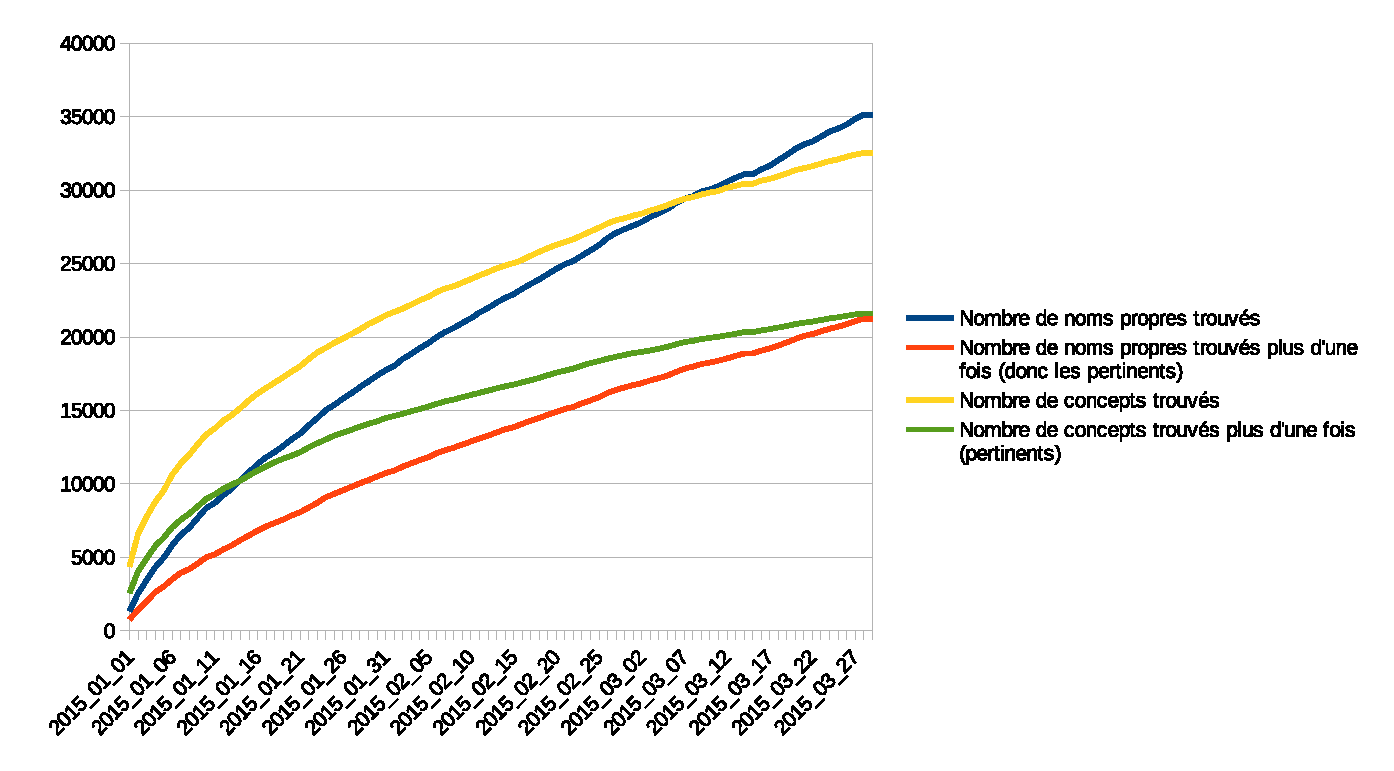
\includegraphics[width=16cm]{./conceptsnoms.eps}
 % conceptsnoms.eps: 0x0 pixel, 300dpi, 0.00x0.00 cm, bb=0 0 653 354
 \caption{\label{fig:conceptsnoms}Évolution en fonction du temps du nombre total de concepts et de noms propres tirés des articles}
\end{figure}



\subsection{WordNet}
%%reprise textuelle

WordNet est une base de données lexicale pour l'anglais, produite par l'université de Princeton.

Nous l'utilisons à travers son interface \pyt{nltk}, pour récupérer des informations sur les mots et les mettre sous forme normale.


\subsection{Conceptnet5}
%%reprise textuelle

Conceptnet (\href{http://conceptnet5.media.mit.edu/}{leur site}) est un projet libre de réseau sémantique représentant des connaissances usuelles, aussi bien de la vie de tous les jours que culturelles et scientifiques. Il fait partie du \ang{Commonsense Computing Initiative} qui relie différents laboratoires, dont le MIT Media Lab, et entreprises.

Il est important de noter que Conceptnet5\index{Concepnet5} est généré à partir de données brutes. Conceptnet5 est relié à DBPedia, une grande partie de ses connaissances provient de Wiktionary, une partie de WordNet.

Nous avons utilisé une partie de code source provenant de \href{https://github.com/commonsense/conceptnet5}{<github>}.


\subsection{Structure de Conceptnet5}
%%reprise textuelle

Conceptnet5\index{Conceptnet5} est un graphe sémantique\index{Graphe sémantique} contenant de l'ordre du million de nœuds et d'ar\^etes.

Les n\oe{}uds sont des mots et de courtes phrases, pas seulement en anglais (bien que pour notre projet, nous utilisions uniquement l'anglais). Les arêtes qui relient ces n\oe{}uds expriment une connaissance, elles contiennent chacune une relation particulière.

Une arête possède aussi une source (d'où provient l'information) et un poids en fonction de cette source, selon l'importance de l'arête.

Une relation concept-arête-concept exprime une assertion\index{Assertion}. Une même assertion peut être exprimée de différentes manières. Conceptnet5 contient 1.6 million d'assertions.

Une assertion peut elle-même être utilisée comme un n\oe{}ud ou comme une arête (on peut avoir des assertions d'assertions).

Les relations valables dans tout langage, pour Conceptnet5, sont par exemple~:
\begin{itemize}
 \item RelatedTo~;
 \item IsA~;
 \item PartOf~;
 \item MemberOf~;
 \item HasA~;
 \item TranslationOf~;
 \item DefinedAs\ldots{}
\end{itemize}

Il en existe beaucoup d'autres.

Comme Conceptnet est construit en partie à l'aide de WordNet, il existe une correspondance entre relations de l'un et de l'autre~:

La correspondance entre relations de WordNet et de Conceptnet est par exemple~:
\begin{itemize}
 \item attribute~: Attribute~;
 \item causes~: Causes~;
 \item classifiedByRegion~: HasContext~;
 \item hyponymOf~: IsA~;
 \item sameVerbGroupAs~: SimilarTo~;
 \item seeAlso~: RelatedTo.
\end{itemize}

Nous avons décidé après coup de conserver ces relations dans le réseau de concepts, et d'en utiliser un sous-ensemble. En effet, elles nous paraissent bien adaptées pour exprimer l'information que nous souhaitons voir contenue dans ce réseau.

\subsection{Détail de l'API (\ang{Application's Programmer Interface})}
%%reprise textuelle

Nous pouvons faire un certain nombre de requêtes à Conceptnet5. Il existe trois types différents de requêtes~:
\begin{itemize}
 \item Lookup~;
 \item Association~;
 \item Search~;
\end{itemize}
Association permet de calculer la proximité entre deux concepts, ou de récupérer une liste de concepts proches d'un concept donné.

Search permet de récupérer une liste d'arêtes (\ang{edges}) entre concepts, selon les paramètres spécifiés (le plus souvent, on impose le concept de départ \ang{start} ou d'arrivée \ang{end}).

Lookup permet d'analyser un concept (on aura par exemple accès à des listes d'arêtes dans lequel il intervient).


\subsection{Utilisation de Conceptnet5}
%%reprise textuelle

Nous utilisons en majorité Association et Search.

Étant donné un concept dont nous savons qu'il doit être étendu, nous utilisons Conceptnet5 pour créer de nouveaux concepts au sein du réseau, et pour ajouter de nouveaux liens. Une première requête de type Search permet d'avoir accès à un certain nombre de liens vers d'autres concepts, qui sont ajoutés (on ne récupère que les plus pertinents). Une requête de type Association permet de créer de nouveaux liens vers d'autres concepts similaires.

Nous ajoutons alors une arête SimilarTo.

\subsection{Freebase}
%%reprise textuelle

Freebase\index{Freebase} est une immense base de données sémantiques qui contient beaucoup d'informations, sur des noms propres notamment. Le projet, repris par Google mais sous une licence qui laisse les données libres d'accès, de téléchargement et d'utilisation, a lui aussi une API, un peu plus complexe que celle de Conceptnet5. Freebase permet notamment de récupérer des informations sur une personne à partir de son nom, et à peu de frais, de vérifier que cette personne existe bel et bien.


\section{Réseau de concepts}

\subsection{Cahier des charges}

Le réseau de concepts\index{Réseau de concepts} est la ``mémoire à long terme'' de notre programme. L'objectif est de disposer d'une représentation souple (sous forme de graphe sémantique) de données conceptuelles qui puissent ensuite être utilisées à mieux comprendre le texte lu.

Étant donné un concept (par exemple \verb|Wayne Rooney|), à quels autres concepts est-il relié et par quelles relations~? Il est essentiel, lorsque le texte ne contient pas suffisamment d'informations ou qu'elles ne sont pas exploitables (on n'a pas toujours ``vu'' à la lecture que Wayne Rooney était un nom propre ou un humain, par exemple), d'insérer ce type de données au cœur du processus de lecture. C'est pourquoi nous avons besoin du réseau de concepts.

D'autre part, nous pouvons exiger du résumé qu'il contienne une information explicite que le texte avait sous-entendu~; par exemple, que Wayne Rooney est un joueur de football. Le réseau devra donc contenir \verb|Wayne Rooney -> isA -> Soccer player|.

Ses prérogatives ont évolué au cours de notre projet. Au début, nous pensions faire reposer une plus grande partie de l'activité de résumé du texte sur lui (notamment par le processus d'activation et le repérage des nœuds activés), alors que celle-ci s'est dirigée ensuite sur le workspace\index{Workspace}.


\subsection{Structure du réseau de concepts}

\begin{definition}[Réseau de concepts]
Ce réseau est au carrefour entre les réseaux sémantiques\index{Graphe sémantique} et les réseaux de neurones. Les nœuds du réseau peuvent être vus comme représentant les concepts\index{Concept}.
\end{definition}

%%reprise textuelle
Le Réseau est constitué de n\oe{}uds. Chaque n\oe{}ud comporte~:
\begin{itemize}
  \item Une étiquette (mot) nommée concept\index{Concept}~;
 \item Une importance conceptuelle (ic) ou profondeur conceptuelle\index{Importance conceptuelle}~;
 \item Une activation (a)\index{Activation} initialement nulle~;
 \item Un certain nombre de liens à d'autres n\oe{}uds.
\end{itemize}

Chaque lien comporte~:
\begin{itemize}
 \item Une proximité conceptuelle\index{Proximité conceptuelle} (ou poids w)~;
 \item Une relation\index{Relation} qui le caractérise, prise sur le modèle de Conceptnet5\index{Conceptnet5}.
\end{itemize}

Ces différentes données numériques (proximité conceptuelle, activation, importance conceptuelle) sont normalisées entre $0$ et $100$.

\begin{figure}[h]
 \centering
 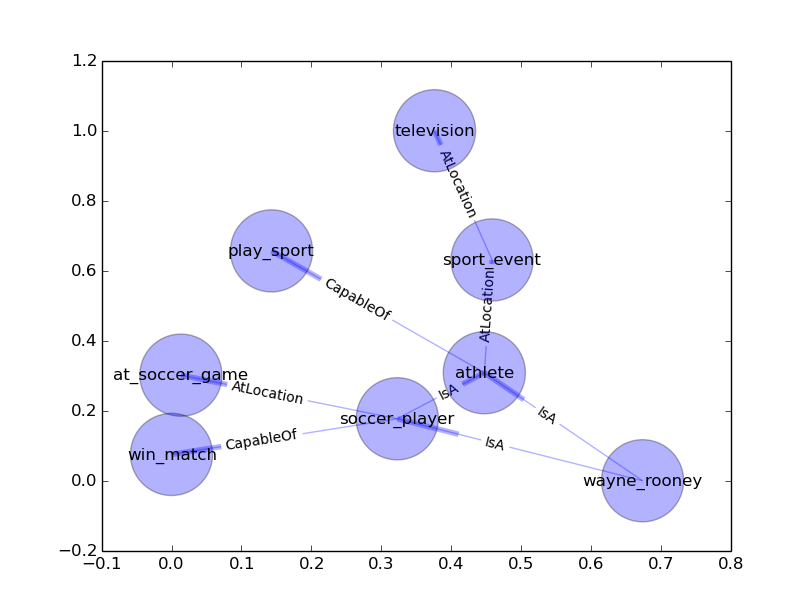
\includegraphics[width=14cm]{./rc_exemple.png}
 % rc_exemple.png: 812x612 pixel, 100dpi, 20.62x15.54 cm, bb=0 0 585 441
 \caption{\label{fig:rc_exemple}Exemple de réseau de concepts}
\end{figure}

\paragraph{}
Sur l'exemple de la figure~\ref{fig:rc_exemple}, nous revoyons les données qui nous intéressent. Les relations entre concepts sont exprimées de manière intuitive (\textit{Wayne Rooney IsA soccer player}, \textit{a soccer player is capableOf winning a match}). Nous ne représentons pas ici les poids, mais nous attendons d'eux qu'ils rendent compte du fait que si Wayne Rooney est effectivement un \textit{athlete}, il est plus pertinent de dire de lui qu'il est un \textit{soccer player}.


\subsection{Propagation d'activation}

Le réseau de concepts est dynamique. Il évolue au cours de la lecture du texte, notamment par un processus d'activation des n\oe{}uds. L'écoulement du temps est donc une donnée importante.

L'activation d'un mot (provoquée par exemple par sa lecture dans un texte) est propagée à tous les n\oe{}uds voisins. Elle permet intuitivement de penser à de nouvelles idées, de compléter l'information du texte si celle-ci est parcellaire.

Sur l'exemple de la figure~\ref{fig:rc_exemple}, l'activation du concept \verb|wayne_rooney| va provoquer dans un premier temps celle de \verb|soccer_player|, \verb|athlete|, mais aussi \verb|play_sport|, \verb|win_match|, etc.

La propagation d'activation doit tenir compte de plusieurs facteurs~: les poids des liens et l'importance conceptuelle des n\oe{}uds. Ainsi, un n\oe{}ud fortement relié à \verb|wayne_rooney| devra être activé plus rapidement et de façon plus importante.

Selon la manière dont nous voulons utiliser le réseau, il y a deux possibilités~:
\begin{itemize}
  \item Ou bien introduire un facteur de désactivation des n\oe{}uds au cours du temps, permettant éventuellement d'arriver à un état d'équilibre~;
 \item Ou bien rester en situation potentielle de déséquilibre (l'activation de chaque n\oe{}ud de la composante connexe ne cesse d'augmenter).
\end{itemize}

La notion de désactivation est assez satisfaisante intuitivement~; il existe en effet des concepts fortement activés mais peu importants, que l'on espère oublier assez rapidement. 

\paragraph{}
Formellement, nous utilisons les formules suivantes, inspirées de [].

\begin{itemize}
  \item Pour l'activation du n\oe{}ud $n$ à l'instant $t+1$~:
\begin{align}
 A_n^{t+1} = A_n^t + D^t + A^t
\end{align}
\item Pour la réactivation de ce n\oe{}ud~:
\begin{align}
 A^t = \sum_{(n' \rightarrow n \text{\ arcs entrants})} W_{(n'\rightarrow  n)} \times A_{n'}^t
\end{align}
\item Pour la désactivation de ce n\oe{}ud~:
\begin{align}
 D^t = \frac{100 \times A^t}{IC_n}
\end{align}
Où le facteur $100$ (modifiable) est dû à la normalisation.
\end{itemize}

\paragraph{}
Nous avons mis un temps plus important à extraire des importances conceptuelles véritablement utiles, et n'avons donc que peu utilisé la désactivation (qui repose sur l'importance conceptuelle). Ces importances conceptuelles ont été finalement calculées en nous inspirant de l'indice TF-IDF\index{TF-IDF}~; ce sera développé dans la partie [].



\subsection{Construction du réseau}
Comme cela a déjà été souligné plus haut, nous nous limitons au domaine du sport, domaine balayé par les articles qui constituent notre première source de données. 

La construction du réseau se déroule en différentes étapes, qui font intervenir quasiment toutes les sources de données de notre projet.


\paragraph{}
Certaines informations sur les éléments du réseau (poids des liens entre concepts notamment) sont relativement faciles à extraire des bases de données utilisées (Freebase, Conceptnet5 comportent déjà de telles informations, qu'il faut simplement renormaliser). En revanche, la seule manière probante d'obtenir une importance conceptuelle est de la calculer nous-mêmes.

Le réseau comporte à la fois des noms propres et des noms communs, des adjectifs, des verbes à l'infinitif~; des termes tout à fait courants (et qui ne sont pas inhérents au sport), comme des termes spécialisés.



\paragraph{Récupération de concepts et de noms}

Nous analysons un certain nombre d'articles, ici 17~000 issus de 7 flux rss différents sur 89 jours (quasiment l'intégralité des données de notre projet).


Nous avons écrit des \ang{tokenizers} adaptés aux contraintes techniques et erreurs d'écriture des données récupérées, qui viennent compléter ceux fournis par \pyt{nltk}.

Pour récupérer les noms propres, nous repérons à l'intérieur d'un article les mots marqués comme noms propres par le POS-tagger\index{Part-of-speech tagger} de \pyt{nltk}. Puis nous concaténons deux noms propres successifs. Enfin, nous retirons de la liste des noms propres ceux qui sont contenus à l'intérieur d'autres. Cette étape, largement sous-estimée au début, est cruciale puisqu'elle évite de considérer ``< nom + prénom >'' et ``<prénom>'' comme deux personnes différentes.

Nous comptons aussi la fréquence d'apparition de chaque nom et de chaque concept. 
On obtient 32~702 concepts et 35~488 noms. En réalité, un tiers d'entre eux sont des mots qui n'apparaissent qu'une seule fois, contenant par exemple des fautes d'orthographe, des néologismes ou résultant d'erreurs de notre part. On obtient par exemple~:
\begin{verbatim}
["aaron cresswell", 78]
["aaron creswell", 1]
\end{verbatim}
Ce qui suggère que dans l'un des articles trouvés, quelqu'un a commis une erreur sur le nom \verb|cresswell|. Nous éliminons donc les mots qui n'apparaissent qu'une fois. Cela nous laisse 27~070 concepts.

\paragraph{Traitement des noms avec Freebase}

Nous n'utilisons l'API Freebase que de fa\c{c}on assez simple. Chaque nom propre donne lieu à une requête. Si celle-ci aboutit, on analyse le résultat et si celui-ci comporte une donnée (exemple~: à l'envoi de \verb|"scott_jamieson"|, on récupère \verb|"soccer_midfielder"|), on ajoute un nouveau nœud correspondant au réseau, et une arête ``<IsA>'' dont le poids dépend du résultat de la requête.

L'importance conceptuelle d'un nom est prise comme importante, par défaut.

\paragraph{Traitement des concepts avec Conceptnet5}

Chaque nouveau concept donne lieu à une requête de type \verb|Lookup|. Nous sélectionnons parmi les résultats les informations les plus pertinentes (en terme de poids, mais aussi en fonction des relations, que nous ne gardons pas toutes~: par exemple, \verb|RelatedTo| n'est pas une relation très pertinente, alors que \verb|IsA| est souvent pertinente).

L'importance conceptuelle allouée à un nouveau n\oe{}ud dépend pour beaucoup de sa fréquence d'apparition dans les articles.


\paragraph{Extension des nœuds du réseau}

Pour étendre les n\oe{}uds du réseau, nous sommes souvent amenés à chercher des liens partant d'un n\oe{}ud donné. Cela est effectué avec des recherches Search. Nous pouvons aussi effectuer des requêtes Association (bien que beaucoup plus lentes) afin d'induire de nouveaux liens avec des concepts similaires.



\paragraph{Suppression des nœuds inutiles}
%%reprise textuelle
Malgré les nombreux paramètres servant à filtrer, les requêtes n'ont pas donné des résultats toujours pertinents. Nous choisissons de retirer du réseau les nœuds faiblement reliés (un seul voisin). Ceux-ci seront de toute fa\c{c}on peu utiles lors de la propagation de l'activation.


\subsection{Exemple de réseau de concepts}

Nous avons eu l'occasion d'effectuer différents essais de construction du réseau de concepts et nous présenterons dans cette sous-section le dernier, qui a donné les résultats les plus intéressants.

\paragraph{Étape 1~: noms propres}

\begin{itemize}
 \item Les requêtes Freebase liées aux noms propres créent 10405 n\oe{}uds dans le réseau, ainsi que 8255 arêtes.
 \item On lance immédiatement des requêtes Search correspondant à tous les n\oe{}uds du réseau sur Conceptnet5, afin d'acquérir plus d'information~: on passe alors à 14103 n\oe{}uds et 28393 arêtes.
\end{itemize}

\paragraph{Étape 2~: concepts}

\begin{itemize}
 \item On lance une requête Lookup sur chaque concept trouvé dans les articles (27070, les noms propres ont déjà été traités)~; on passe alors à 35780 n\oe{}uds et 56942 arêtes. Pour le moment, 18762 n\oe{}uds sont certains d'être conservés (ce sont des résultats primaires de requêtes positives).
\end{itemize}


\paragraph{Étape 3~: Extension et élagage du réseau}

\begin{itemize}
 \item On étend alors l'ensemble des n\oe{}uds encore litigieux (17018), en essayant de créer des liens vers des n\oe{}uds déjà existants, augmentant ainsi la connectivité du réseau. On passe à 76497 arêtes.
 \item On regarde quels n\oe{}uds sont bien reliés à leur voisins, après cette opération. Au total, 28583 n\oe{}uds semblent prometteurs.
 \item On supprime les autres n\oe{}uds. On obtient un réseau avec 28583 n\oe{}uds et 69307 arêtes.
\end{itemize}



\subsection{Choix de programmation du réseau de concepts}

Le réseau est enregistré sous forme de JSON Stream\index{JSON Stream}, un type de données repris à Conceptnet5, qui permet sans contrainte technique majeure de l'écrire sous forme facilement lisible par un utilisateur extérieur. Le nombre de nœuds étant resté raisonnable, nous n'avons pas eu à abandonner le package \pyt{networkx} qui nous permet de le représenter en mémoire sous forme de graphe.

\paragraph{}
Nous avons parallélisé les requêtes afin de les effectuer dans un temps raisonnable, même si l'opération de construction du réseau reste longue dans son ensemble (plus d'une heure) et que les quantités de données mises en jeu suggèrent qu'une utilisation différente, notamment de Conceptnet5 (téléchargement et recherche dans la base de données de façon locale), pourrait être faite.



\section{TF-IDF}

\section{À intégrer}

\subsection{Résolution de pronoms}

Le but de la résolution de pronoms\index{Résolution de pronoms} est, étant donné une phrase qui peut être par exemple~:

\begin{verbatim}
 Sepp_+_Blatter is the favourite to win a Fifa race he vowed he would not stand for.
\end{verbatim}
de rapporter chaque pronom à un groupe nominal. Ici, les deux pronoms que l'on repère (``he'') se rapportent évidemment à \verb|Sepp_+_Blatter|.

Nous disposons pour nous aider des données fournies par l'analyseur syntaxique de Systran. En voici une liste non exhaustive~:
\begin{itemize}
 \item POS\index{Part-of-speech}
 \item Type grammatical de chaque mot~: nom propre, acronyme, verbe, auxiliaire, préposition\ldots{}
 \item Différents liens entre les mots~: adjectif relié à un nom, article\ldots{}
\end{itemize}


\subsubsection{Étape 1}
On commence par trouver l'ensemble des groupes nominaux. Nous avons deux choix~:
\begin{itemize}
 \item Ou bien les trouver tous~;
 \item Ou bien se limiter d'emblée à ceux qui ont leurs chances.
\end{itemize}

Nous prenons d'abord le deuxième choix~: l'analyseur de Systran nous indique en particulier, étant donné un mot, s'il est objet ou sujet d'un verbe. Nous considérons donc, dans un premier temps, que les noms concernés sont les noms principaux et que tous les groupes nominaux qui nous intéressent se construisent autour d'eux.

Après expérience, nous avons étendu le ``droit'' de créer un groupe nominal à de simples compléments d'objet, constatant qu'ils apparaissaient eux aussi.


\subsubsection{Étape 2}
On considère maintenant l'ensemble des pronoms.

Pour un pronom situé à une position donnée, les groupes nominaux\index{Groupe nominal} potentiels font l'objet d'un classement, relatif à un score, que nous calculons de la manière suivante~:

\begin{itemize}
 \item Un candidat a le droit d'être situé dans une phrase précédente (sous une limite fixée à 2 ou 3). Plus il est éloigné du pronom, plus son score diminue. S'il est après le pronom, son score diminue drastiquement (voire $-\infty$).
 \item Le candidat doit vérifier certaines correspondances avec le pronom~: en particulier, il doit avoir le même genre et le même nombre. Si c'est vérifié, le score augmente. Sinon, le score diminue. Cette information n'est pas tout le temps disponible. En revanche, on sait parfois si le groupe nominal concerné (son nom principal) est un humain ou non.
 \item On a parfois (notamment avec le pronom ``that'') de manière directe l'information de l'antécédent. L'antécédent désigné doit alors gagner un score énorme (voire $+\infty$, mais l'analyseur de Systran n'est pas infaillible).
 \item Un groupe nominal qui apparaît au début d'une phrase doit, quels que soient les pronoms, avoir un meilleur score. Les noms propres apparaissent souvent au début de la phrase pour être ensuite rappelés par des pronoms, c'est d'ailleurs le cas dans l'exemple ci-dessus.
 \item Un groupe nominal répété gagne également en score.
 \item Un groupe nominal précédé d'une préposition perd en score.
 \item Un groupe nominal sujet gagne en score, et un groupe objet perd en score. 
 \item Un groupe nominal comportant un article indéfini perd en score.
 \item Un groupe nominal comportant un nom propre gagne en score.
\end{itemize}

Ces différentes exigences satisfont à un impératif de simplicité. On cherche ensuite à balancer le mieux possible les augmentations/diminutions de score afin de maximiser la pertinence des résultats.

Nous nous inspirons pour cette méthode de ``<Robust pronoun resolution with limited knowledge>'', pour sa simplicité et son adaptabilité quant aux données dont nous disposons.


%%%%%%%%%%%%%%%%%%%%%%%%%%%%%%%%%%%%%%%%%%%%%%%%%%%%%%%%

%%%%%%%%%%%%%%%%%%%%%%%%%%%%%%%%%%%%%%%%%%%%%%%%%%%%%%%ù

%%%%%%%%%%%%%%%%%%%%%%%%%%%%%%%%%%%%%%%%%%%%%%%%%%%%%%%ù

\section{Traitement du réseau}

Le réseau de concepts représente, comme nous l'avons déjà dit, la connaissance \textit{a priori} de notre programme sur le domaine étudié. Pour étudier un texte particulier, il s'agit maintenant de faire agir ce texte sur nos connaissances et d'interpréter l'effet que cette lecture a.

Deux méthodes ont été envisagées~: la première étudiait, essentiellement, la différence entre l'état du réseau de concepts avant et après la lecture et devait en déduire les faits importants. La seconde, qui a finalement été retenue, s'appuie sur une activation des concepts dans le réseau, puis une instanciation des concepts fortement activés dans un espace de travail appelé \textit{workspace}\index{Workspace}. Ces concepts instanciés sont par la suite capable d'effectuer des tâches plus complexes relatives à la compréhension du texte.

Quelle que soit la méthode employée, une analyse syntaxique\index{Analyse syntaxique} préalable du texte est nécessaire pour rendre compte de sa compréhension et utiliser au mieux notre réseau de connaissances.

\subsection{Workspace}\index{Workspace}
Le Workspace est une zone où on va stocker des structures formées à partir de concepts et travailler dessus. Par opposition au réseau de concepts, qui représente une connaissance relativement figée du monde, ces structures visent à représenter la compréhension que l'on a pu acquérir du texte.
Par exemple, un type de structure rencontré dans le Workspace serait un graphe décrivant l'évolution de l'état d'un objet au fur et à mesure du temps, d'après ce qu'on a pu extraire du texte.

Au fur et à mesure que l'on découvre les concepts pertinents par rapport au texte grâce au réseau de concepts, on va les ajouter (instancier) au Workspace afin de pouvoir travailler dessus. Ensuite, au moyen de diverses méthodes appelées Workers\index{Worker}, on va chercher à les rassembler en des structures porteuses de sens. Les Workers pourront extraire de l'information grâce au texte, sa structure grammaticale, les liens du réseau de connaissances et les structures déjà présentes dans le Workspace.

Par exemple, il y aurait un Worker capable de reconnaître l'identité d'un objet dans le texte. Lorsqu'un concept est instancié dans le Workspace, il cherchera à détecter si ce concept fait référence à un objet récurrent dans le texte, comme par exemple une personne.
En reprenant l'exemple précédent, il y aurait aussi un Worker\index{Worker} capable de repérer dans la phrase les descriptions de succession temporelle, et qui créerait les structures dans le Workspace qui reflètent cette évolution. 


\subsection{Analyse syntaxique}\index{Analyse syntaxique}

Cette partie ne constituant pas le c\oe{}ur de notre psc, nous avons décidé d'utiliser un outil déjà codé, faisant partie de la plus grande librairie libre \pyt{nltk}\index{Natural Language ToolKit}.

\subsubsection{Description algorithmique d'une grammaire}\index{Grammaire}
Une grammaire peut être décrite informatiquement de manière très simple. En effet, on peut la voir comme~:
\begin{itemize}
	\item Un ensemble de classes terminales (verbe, nom par exemple) associées à une liste de mots ou éventuellement d'expressions
	\item Un ensemble de règles, souvent sous la forme d'une reconnaissance de motifs, permettant de découper une phrase en plusieurs éléments (et finalement en unités syntaxiques élémentaires).
\end{itemize}

Il y a par conséquent deux manières pour une grammaire d'être incomplète~: soit elle ne connaît pas assez de vocabulaire (manque d'éléments dans les cas terminaux), soit elle ne connaît pas assez de règles. La première faille est assez facile à combler par des requêtes vers WordNet\index{WordNet} (et par ailleurs un outil automatique est inclus dans \pyt{nltk}\index{Natural Language ToolKit})~; il est en revanche assez indispensable d'avoir une grammaire complète en termes de règles car il est beaucoup plus difficile d'inventer des manières de découper une phrase.

\subsubsection{\'Etat du texte en fin d'analyse}
Les grammaires \pyt{nltk} sont classées selon la forme de leur sortie. Elles attendent la liste des mots dans l'ordre dans lequel ils apparaissent dans le texte à étudier, accompagnés d'une liste de classes possibles pour ces mots. En sortie, on peut trouver~:

\begin{itemize}
	\item Un arbre représentant une structure grammaticale possible pour la phrase.
	\item La liste de tous les arbres pouvant représenter la structure grammaticale de la phrase.
	\item La liste de tous les arbres pouvant représenter la structure grammaticale de la phrase, et pour chaque arbre une mesure de la vraisemblance de cette structure.
\end{itemize}

Il y a une grande différence entre les n\oe{}uds non terminaux des arbres en sortie et leurs feuilles. En effet, ces dernières seront les unités syntaxiques présentes à l'origine dans la phrase, tandis que les n\oe{}uds internes représentent la classe grammaticale des bouts de phrases représentés par les sous-arbres dont ils sont la racine.

%Un exemple serait sûrement le bienvenu, je vais voir si je me chauffe pour faire un ParseTree a l'air plausible. (Antonin)
%Cela étant n'hésitez pas à vous chauffer vous aussi.

Les n\oe{}uds internes sont en nombre fini et leurs étiquettes dépendent de si on considère des grammaires sans contexte (capables de séparer des composants autour d'un verbe) ou des grammaires à dépendance (dont le but est d'identifier le sujet et les compléments du verbe central).


\section{Suites envisagées}

Dans l'ensemble le projet avance avec peu de retard sur le plan prévisionnel écrit en novembre dernier. Le réseau de concepts est prêt à être utilisé et notre attention pourra se reporter sur le développement du \textit{workspace}\index{Workspace} et du déploiement de l'analyse syntaxique.\index{Analyse syntaxique}

Cette dernière, que nous avions prise pour à peu près acquise, s'avère requérir plus de travail que prévu. En effet, l'outil que nous avions prévu d'utiliser --- les ``grammaires'' \pyt{nltk}\index{Grammaire} --- soufrent d'un manque de souplesse rédhibitoire. Elles doivent en particulier connaître en avance tous les mots de la phrase pour pouvoir l'analyser, ce qui même en construisant un dictionnaire exhaustif --- qui n'existe pas à l'heure actuelle --- est très limitant pour peu qu'une phrase contienne un néologisme où un nom propre peu connu (voire une simple faute d'orthographe). Nous penchons donc plus actuellement pour des méthodes statistiques plus souples, mais aussi plus difficiles à appréhender.

\vspace{1\baselineskip}

La planification pour le reste du projet est la suivante~:
\begin{description}
	\item[Février~: ]Mise en place de l'analyseur syntaxique. Responsables~: Antonin Angibault, Théophane Hufschmitt, Sarah Fernandes-Pinto-Fachada.
	\item[Février~: ]Fin de la spécification du contenu du \textit{workspace}.
	\item[Février-Avril~: ]Implémentation du \textit{workspace} (donc, essentiellement, de ce qui manque à l'algorithme de résumé pour fonctionner).
	\item[Avril~: ]Génération de résumé et évaluation de ceux-ci.
\end{description}

Les différences essentielles avec la planification initiale proviennent de la complexité inattendue de la grammaire. En revanche, le temps d'exécution prévu pour la production d'un résumé d'article étant long, nous produirons finalement peu de résumés à évaluer, cela nous permet donc de les évaluer à la main et de gagner du temps sur cette partie de la planification initiale.

Globalement nous pensons être capables de mener le projet à bien comme prévu. Les sections suivantes décrivent les points prêts à être mis en place.

\subsection{Apprentissage du réseau de concepts}
Le réseau de concept représente un \textit{a priori} sur le monde de notre programme. Il est donc normal que cette structure évolue au fur et à mesure des textes lus.

Les fonctions de construction du réseau peuvent sans mal être appelées après la génération du résumé pour y apporter des modifications pérennes.

\subsection{\'Evaluation des résumés}
Le faible nombre de résumés que nous prévoyons de produire nous permettra d'utiliser la méthode la plus simple parmi celles qui étaient mentionnées dans la proposition détaillée~: la comparaison à un résumé déclaré bon car produit par un humain.

L'idée est la suivante~: l'un de nous résumera un texte, nous emploierons notre programme pour résumer le même texte, et enfin nous utiliserons un simple algorithme statistique (basé sur TF-IDF) pour résumer ce même texte. Nous comparerons ensuite ces résumés du point de vue de l'information qu'ils contiennent~: sont-ils des images assez fidèles du document original~?

Compte-tenu de la simplicité de l'algorithme statistique, nous espérons que le résumé produit par notre programme se situera quelque part entre le résumé statistique et le résumé humain.


\subsubsection{Algorithme statistique}
Les analyses statistiques sont basé sur la méthode TF-IDF qui permet d'évaluer l'importance d'un terme contenu dans un document, relativement à une collection ou un corpus. L'idée principale ici est de donner à chaque terme une indice d'importance et éventuellement à chaque phrase. Puis faire un résumé en tirant les phrases plus importantes.


\subsubsection{Qualité de résumé}
La qualité de résumé par la méthode TF-IDF est peu optimale. En effet, avec un regroupement simple de phrases, on perd beaucoup d'information contextuel. Et comme une phrase sans contexte est souvent peu compréhensible, c'est toujours difficile de lire ces résumés.
En revanche, pour la recherche des mots-clés, la méthode TF-IDF est assez efficace. Nous avous remarqués qu'à partir de ces mots-clés, à l'aide d'une méthode synthétique, nous pouvons construire des phrases plus claires et éventuellement faire un résumé du texte.
 

\section{Références bibliographiques}

\begin{quotation}
 This work includes data from ConceptNet 5, which was compiled by the Commonsense Computing Initiative. ConceptNet 5 is freely available under the Creative Commons Attribution-ShareAlike license (CC BY SA 3.0) from http://conceptnet5.media.mit.edu. The included data was created by contributors to Commonsense Computing projects, contributors to Wikimedia projects, Games with a Purpose, Princeton University's WordNet, DBPedia, OpenCyc, and Umbel.
\end{quotation}

\nocite{*}
\printbibliography{}

\appendix

\printindex


\end{document}
